% Options for packages loaded elsewhere
\PassOptionsToPackage{unicode}{hyperref}
\PassOptionsToPackage{hyphens}{url}
%
\documentclass[
]{article}
\usepackage{lmodern}
\usepackage{amssymb,amsmath}
\usepackage{ifxetex,ifluatex}
\ifnum 0\ifxetex 1\fi\ifluatex 1\fi=0 % if pdftex
  \usepackage[T1]{fontenc}
  \usepackage[utf8]{inputenc}
  \usepackage{textcomp} % provide euro and other symbols
\else % if luatex or xetex
  \usepackage{unicode-math}
  \defaultfontfeatures{Scale=MatchLowercase}
  \defaultfontfeatures[\rmfamily]{Ligatures=TeX,Scale=1}
\fi
% Use upquote if available, for straight quotes in verbatim environments
\IfFileExists{upquote.sty}{\usepackage{upquote}}{}
\IfFileExists{microtype.sty}{% use microtype if available
  \usepackage[]{microtype}
  \UseMicrotypeSet[protrusion]{basicmath} % disable protrusion for tt fonts
}{}
\makeatletter
\@ifundefined{KOMAClassName}{% if non-KOMA class
  \IfFileExists{parskip.sty}{%
    \usepackage{parskip}
  }{% else
    \setlength{\parindent}{0pt}
    \setlength{\parskip}{6pt plus 2pt minus 1pt}}
}{% if KOMA class
  \KOMAoptions{parskip=half}}
\makeatother
\usepackage{xcolor}
\IfFileExists{xurl.sty}{\usepackage{xurl}}{} % add URL line breaks if available
\IfFileExists{bookmark.sty}{\usepackage{bookmark}}{\usepackage{hyperref}}
\hypersetup{
  pdftitle={Assessment of Mental Health Need Before, During, and After COVID-19},
  pdfauthor={Jensen Hu},
  hidelinks,
  pdfcreator={LaTeX via pandoc}}
\urlstyle{same} % disable monospaced font for URLs
\usepackage[margin=1in]{geometry}
\usepackage{longtable,booktabs}
% Correct order of tables after \paragraph or \subparagraph
\usepackage{etoolbox}
\makeatletter
\patchcmd\longtable{\par}{\if@noskipsec\mbox{}\fi\par}{}{}
\makeatother
% Allow footnotes in longtable head/foot
\IfFileExists{footnotehyper.sty}{\usepackage{footnotehyper}}{\usepackage{footnote}}
\makesavenoteenv{longtable}
\usepackage{graphicx,grffile}
\makeatletter
\def\maxwidth{\ifdim\Gin@nat@width>\linewidth\linewidth\else\Gin@nat@width\fi}
\def\maxheight{\ifdim\Gin@nat@height>\textheight\textheight\else\Gin@nat@height\fi}
\makeatother
% Scale images if necessary, so that they will not overflow the page
% margins by default, and it is still possible to overwrite the defaults
% using explicit options in \includegraphics[width, height, ...]{}
\setkeys{Gin}{width=\maxwidth,height=\maxheight,keepaspectratio}
% Set default figure placement to htbp
\makeatletter
\def\fps@figure{htbp}
\makeatother
\setlength{\emergencystretch}{3em} % prevent overfull lines
\providecommand{\tightlist}{%
  \setlength{\itemsep}{0pt}\setlength{\parskip}{0pt}}
\setcounter{secnumdepth}{-\maxdimen} % remove section numbering

\title{Assessment of Mental Health Need Before, During, and After COVID-19}
\author{Jensen Hu}
\date{}

\begin{document}
\maketitle

\hypertarget{purpose}{%
\subsection{Purpose}\label{purpose}}

The purpose of this assessment is to identify areas of potentially
increased mental health need as a result of COVID-19 in NYC. The
resulting aim is to route public health efforts and mental health
resources to those identified areas of highest need.

\hypertarget{background-of-datasets}{%
\subsection{Background of Datasets}\label{background-of-datasets}}

\textbf{For this assessment, we will use the CDC's Social Vulnerability
Index along with the child opportunity index to establish the baseline
mental health need in NYC. COVID19 related data will then be added onto
this baseline as a ``COVID19 Layer'' to identify those areas of
increased mental health need in the context of COVID19}

\hypertarget{social-vulnerability-index-svi}{%
\paragraph{\texorpdfstring{\textbf{Social Vulnerability Index
(SVI)}}{Social Vulnerability Index (SVI)}}\label{social-vulnerability-index-svi}}

\begin{itemize}
\tightlist
\item
  \textbf{Background}: In the context of the global COVID-19 pandemic,
  ``SVI data can be used to identify communities that will need
  continued support to recover following an emergency or natural
  disaster, and allocate emergency preparedness funding by community
  need.'' As seen in current events, COVID19 disproportionately affects
  Black and Hispanic communities. It is evident that public health
  institutions not only factor in, but lead with the social determinants
  of health -- which contribute to racial inequities in health-- when
  planning and executing emergency resource allocation during and after
  COVID19.
\end{itemize}

\hypertarget{exploration-of-social-vulnerability-index-svi}{%
\paragraph{\texorpdfstring{\textbf{Exploration of Social Vulnerability
Index
(SVI)}}{Exploration of Social Vulnerability Index (SVI)}}\label{exploration-of-social-vulnerability-index-svi}}

SVI consists of 15 census variables organized into 4 different themes:
Socioeconomic Status (RPL\_THEME1), Household Composition \& Disability
(RPL\_THEME2), Minority Status \& Language (RPL\_THEME3), Housing \&
Transportation (RPL\_THEME4) and an overall summary (RPL\_THEMES). These
themes are measured in percentile rank. A higher percentile rank
represents greater vulnerability, with a percentile rank of 0.00 meaning
the least vulnerable and 1.00 meaning the most vulnerable.
Reference:\url{https://svi.cdc.gov/Documents/Data/2016_SVI_Data/SVI2016Documentation.pdf}

These rankings have been alloted by census tract (GEOID)-- ``uniquely
numbered subdivisions of a county, representing a neighborhood averaging
about 4,000 inhabitants.'' NYC has 5 different counties (``New York'',
``Kings'', ``Bronx'', ``Richmond'', ``Queens'') which have been
subdivided into 2,166 census tracts. To provide a frame of reference,
census tracts are more granular than zip codes. There are 178 zip codes
in NYC.

To begin, we will review SVI data by NY county.

\hypertarget{review-of-svi-data-by-nyc-county}{%
\subparagraph{\texorpdfstring{\textbf{Review of SVI Data by NYC
County}}{Review of SVI Data by NYC County}}\label{review-of-svi-data-by-nyc-county}}

\begin{longtable}[]{@{}lllrrrrr@{}}
\toprule
COUNTY & FIPS & LOCATION & RPL\_THEME1 & RPL\_THEME2 & RPL\_THEME3 &
RPL\_THEME4 & RPL\_THEMES\tabularnewline
\midrule
\endhead
Richmond & 36085 & Richmond County, New York & 0.2951 & 0.1967 & 0.8852
& 0.7049 & 0.5410\tabularnewline
New York & 36061 & New York County, New York & 0.5738 & 0.0164 & 0.9508
& 0.9672 & 0.6393\tabularnewline
Queens & 36081 & Queens County, New York & 0.7049 & 0.0328 & 0.9836 &
0.7213 & 0.7377\tabularnewline
Kings & 36047 & Kings County, New York & 0.9016 & 0.3770 & 0.9672 &
0.8525 & 0.9180\tabularnewline
Bronx & 36005 & Bronx County, New York & 1.0000 & 0.8033 & 1.0000 &
0.9508 & 1.0000\tabularnewline
\bottomrule
\end{longtable}

At a glance, the Bronx county has the highest overall social
vulnerability (RPL\_THEMES=1.000) followed by Kings county
(RPL\_THEMES=0.918). This seems to indicate that these two counties are
likely to be substantially impacted by COVID19 and need priority
allocation of emergency resources.

\hypertarget{mapping-svi-data-by-county}{%
\subparagraph{\texorpdfstring{\textbf{Mapping SVI data by
County}}{Mapping SVI data by County}}\label{mapping-svi-data-by-county}}

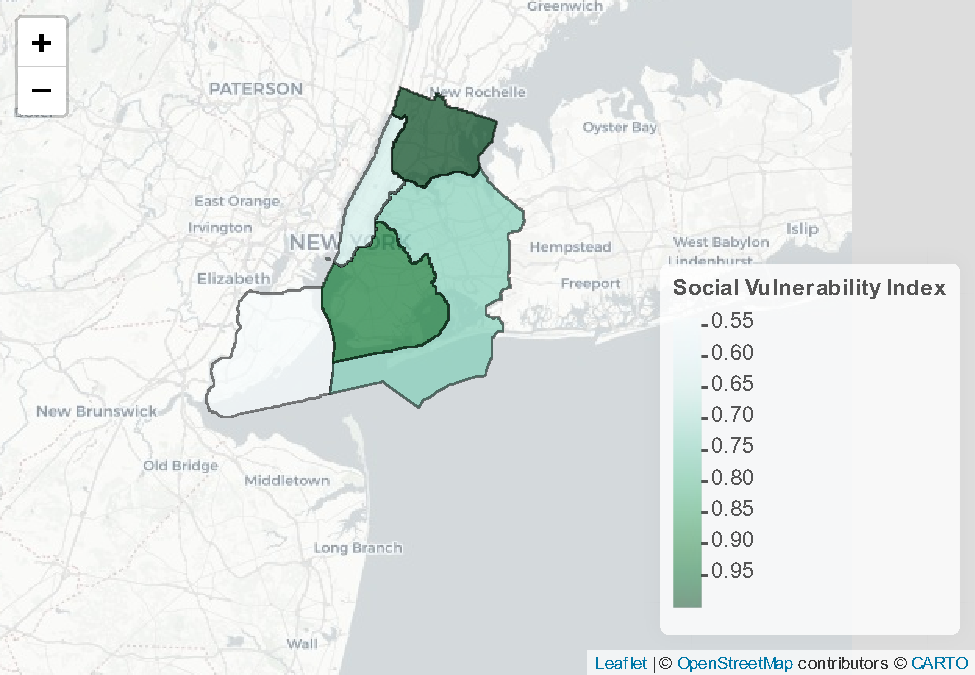
\includegraphics{leaflet_files/figure-latex/unnamed-chunk-4-1.pdf}

Now, let's take a look at how COVID19 has impacted NYC counties to date:

\begin{verbatim}
## Parsed with column specification:
## cols(
##   BOROUGH_GROUP = col_character(),
##   COVID_CASE_COUNT = col_double(),
##   COVID_CASE_RATE = col_double()
## )
\end{verbatim}

\begin{longtable}[]{@{}lrrl@{}}
\toprule
BOROUGH\_GROUP & COVID\_CASE\_COUNT & COVID\_CASE\_RATE &
COUNTY\tabularnewline
\midrule
\endhead
The Bronx & 36382 & 2472.77 & Bronx\tabularnewline
Brooklyn & 42380 & 1562.41 & Kings\tabularnewline
Manhattan & 19837 & 1053.67 & New York\tabularnewline
Queens & 49559 & 1980.51 & Queens\tabularnewline
Staten Island & 11635 & 2315.73 & Richmond\tabularnewline
Citywide & 159865 & NA & NA\tabularnewline
\bottomrule
\end{longtable}

The above contains cumulative, age adjusted rates of confirmed cases per
100,000 people, by NYC borough of residence. We can see that The Bronx
(Bronx County) and Staten Island (Richmond County) have higher COVID
case rates in relation to all other counties. Assuming COVID case rate
is an indicator of COVID impact, let's add in COVID data into the
current SVI rankings.

Note: I don't think it's this easy.

\hypertarget{adding-covid-data-into-percent-ranking-in-svi}{%
\subparagraph{\texorpdfstring{\textbf{Adding COVID DATA into Percent
Ranking in
SVI}}{Adding COVID DATA into Percent Ranking in SVI}}\label{adding-covid-data-into-percent-ranking-in-svi}}

\begin{verbatim}
##  [1] "COUNTY"           "FIPS"             "LOCATION"         "RPL_THEME1"      
##  [5] "RPL_THEME2"       "RPL_THEME3"       "RPL_THEME4"       "SPL_THEMES"      
##  [9] "RPL_THEMES"       "BOROUGH_GROUP"    "COVID_CASE_COUNT" "COVID_CASE_RATE" 
## [13] "covid_rank"       "adj_SPL"          "svi_covid_rank"
\end{verbatim}

\begin{longtable}[]{@{}llrrrrr@{}}
\toprule
\begin{minipage}[b]{0.09\columnwidth}\raggedright
COUNTY\strut
\end{minipage} & \begin{minipage}[b]{0.13\columnwidth}\raggedright
BOROUGH\_GROUP\strut
\end{minipage} & \begin{minipage}[b]{0.11\columnwidth}\raggedleft
SPL\_THEMES\strut
\end{minipage} & \begin{minipage}[b]{0.15\columnwidth}\raggedleft
COVID\_CASE\_RATE\strut
\end{minipage} & \begin{minipage}[b]{0.11\columnwidth}\raggedleft
covid\_rank\strut
\end{minipage} & \begin{minipage}[b]{0.08\columnwidth}\raggedleft
adj\_SPL\strut
\end{minipage} & \begin{minipage}[b]{0.14\columnwidth}\raggedleft
svi\_covid\_rank\strut
\end{minipage}\tabularnewline
\midrule
\endhead
\begin{minipage}[t]{0.09\columnwidth}\raggedright
Richmond\strut
\end{minipage} & \begin{minipage}[t]{0.13\columnwidth}\raggedright
Staten Island\strut
\end{minipage} & \begin{minipage}[t]{0.11\columnwidth}\raggedleft
7.4917\strut
\end{minipage} & \begin{minipage}[t]{0.15\columnwidth}\raggedleft
2315.73\strut
\end{minipage} & \begin{minipage}[t]{0.11\columnwidth}\raggedleft
0.75\strut
\end{minipage} & \begin{minipage}[t]{0.08\columnwidth}\raggedleft
8.2417\strut
\end{minipage} & \begin{minipage}[t]{0.14\columnwidth}\raggedleft
0.25\strut
\end{minipage}\tabularnewline
\begin{minipage}[t]{0.09\columnwidth}\raggedright
New York\strut
\end{minipage} & \begin{minipage}[t]{0.13\columnwidth}\raggedright
Manhattan\strut
\end{minipage} & \begin{minipage}[t]{0.11\columnwidth}\raggedleft
7.8524\strut
\end{minipage} & \begin{minipage}[t]{0.15\columnwidth}\raggedleft
1053.67\strut
\end{minipage} & \begin{minipage}[t]{0.11\columnwidth}\raggedleft
0.00\strut
\end{minipage} & \begin{minipage}[t]{0.08\columnwidth}\raggedleft
7.8524\strut
\end{minipage} & \begin{minipage}[t]{0.14\columnwidth}\raggedleft
0.00\strut
\end{minipage}\tabularnewline
\begin{minipage}[t]{0.09\columnwidth}\raggedright
Queens\strut
\end{minipage} & \begin{minipage}[t]{0.13\columnwidth}\raggedright
Queens\strut
\end{minipage} & \begin{minipage}[t]{0.11\columnwidth}\raggedleft
8.1966\strut
\end{minipage} & \begin{minipage}[t]{0.15\columnwidth}\raggedleft
1980.51\strut
\end{minipage} & \begin{minipage}[t]{0.11\columnwidth}\raggedleft
0.50\strut
\end{minipage} & \begin{minipage}[t]{0.08\columnwidth}\raggedleft
8.6966\strut
\end{minipage} & \begin{minipage}[t]{0.14\columnwidth}\raggedleft
0.50\strut
\end{minipage}\tabularnewline
\begin{minipage}[t]{0.09\columnwidth}\raggedright
Kings\strut
\end{minipage} & \begin{minipage}[t]{0.13\columnwidth}\raggedright
Brooklyn\strut
\end{minipage} & \begin{minipage}[t]{0.11\columnwidth}\raggedleft
9.9672\strut
\end{minipage} & \begin{minipage}[t]{0.15\columnwidth}\raggedleft
1562.41\strut
\end{minipage} & \begin{minipage}[t]{0.11\columnwidth}\raggedleft
0.25\strut
\end{minipage} & \begin{minipage}[t]{0.08\columnwidth}\raggedleft
10.2172\strut
\end{minipage} & \begin{minipage}[t]{0.14\columnwidth}\raggedleft
0.75\strut
\end{minipage}\tabularnewline
\begin{minipage}[t]{0.09\columnwidth}\raggedright
Bronx\strut
\end{minipage} & \begin{minipage}[t]{0.13\columnwidth}\raggedright
The Bronx\strut
\end{minipage} & \begin{minipage}[t]{0.11\columnwidth}\raggedleft
11.8525\strut
\end{minipage} & \begin{minipage}[t]{0.15\columnwidth}\raggedleft
2472.77\strut
\end{minipage} & \begin{minipage}[t]{0.11\columnwidth}\raggedleft
1.00\strut
\end{minipage} & \begin{minipage}[t]{0.08\columnwidth}\raggedleft
12.8525\strut
\end{minipage} & \begin{minipage}[t]{0.14\columnwidth}\raggedleft
1.00\strut
\end{minipage}\tabularnewline
\bottomrule
\end{longtable}

Based on the new ``svi\_covid\_rank'', we can see that Bronx and Kings
county still hold their rank as the highest in social vulnerability in
the context of COVID.

\hypertarget{mapping-covid-adjusted-svi-data-by-county}{%
\subparagraph{\texorpdfstring{\textbf{Mapping COVID adjusted SVI data by
County}}{Mapping COVID adjusted SVI data by County}}\label{mapping-covid-adjusted-svi-data-by-county}}

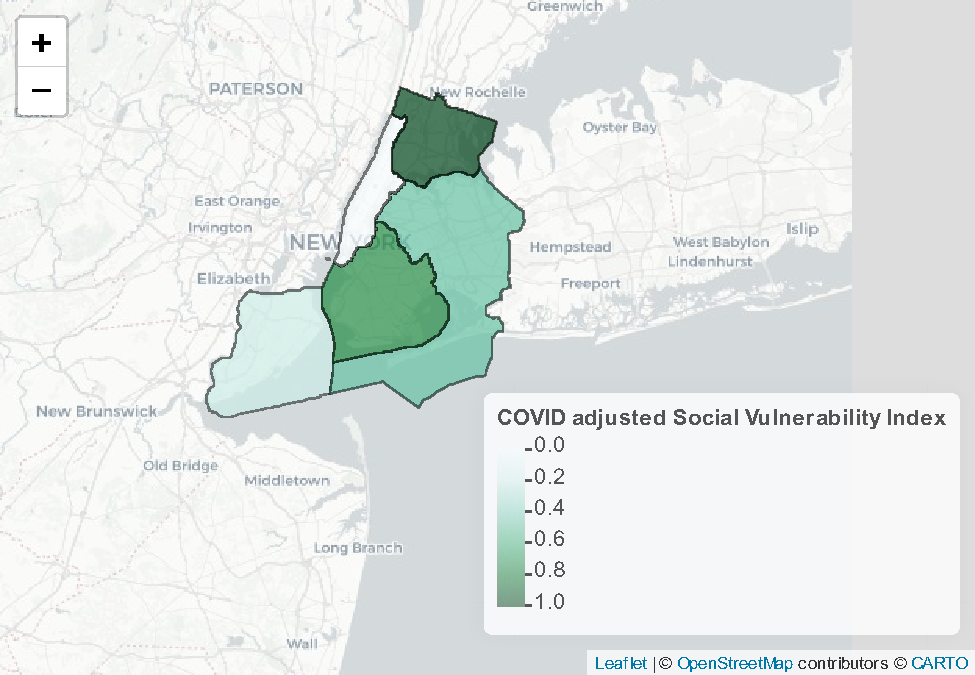
\includegraphics{leaflet_files/figure-latex/unnamed-chunk-7-1.pdf}

\hypertarget{zip-code-cleantransform-178-zip-codes-in-nyc}{%
\paragraph{ZIP CODE CLEAN/TRANSFORM \#178 zip codes in
nyc}\label{zip-code-cleantransform-178-zip-codes-in-nyc}}

\hypertarget{leaflet1---svi-by-census-tract}{%
\paragraph{Leaflet\#1 - SVI by Census
Tract}\label{leaflet1---svi-by-census-tract}}

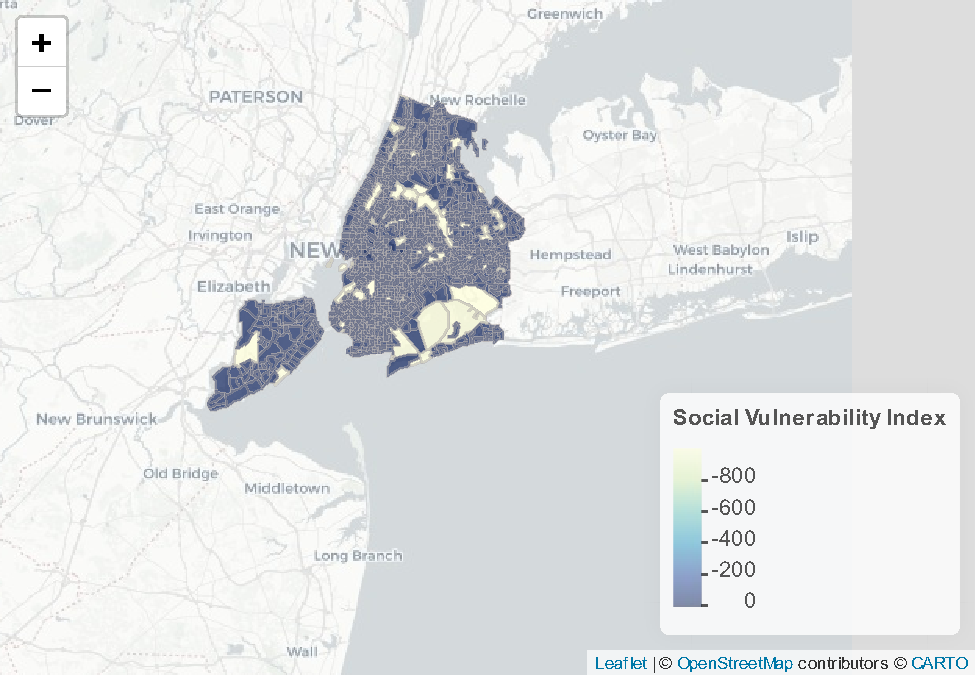
\includegraphics{leaflet_files/figure-latex/unnamed-chunk-10-1.pdf}

\hypertarget{leaflet2---nyc-zips}{%
\paragraph{Leaflet\#2 - NYC ZIPS}\label{leaflet2---nyc-zips}}

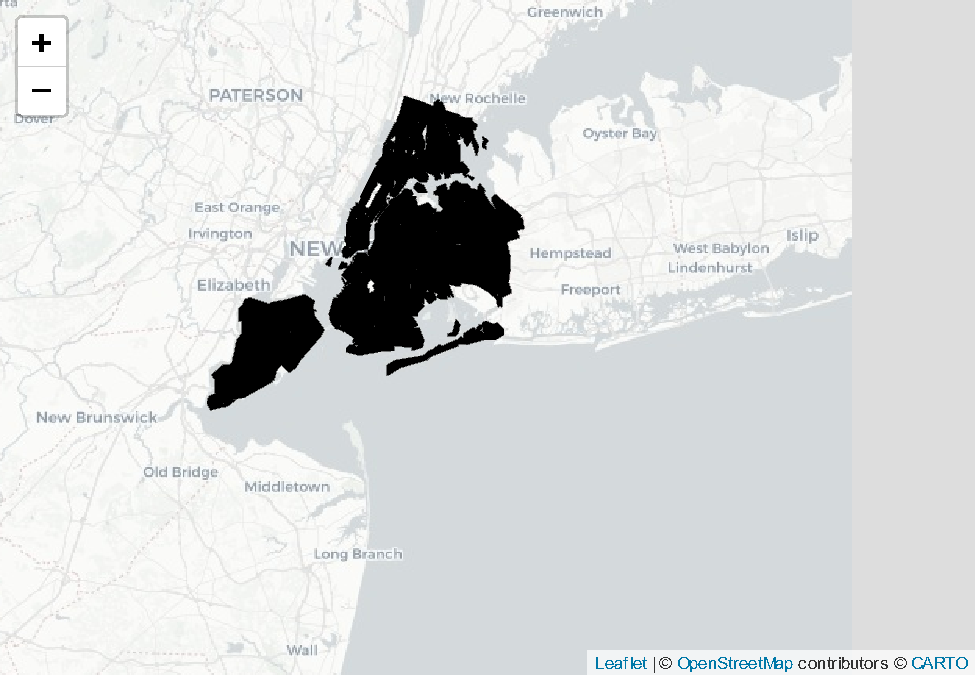
\includegraphics{leaflet_files/figure-latex/unnamed-chunk-11-1.pdf}
\#\#\#\# Leaflet\#3 - NYC ZIPS + COVID19 \% Positive
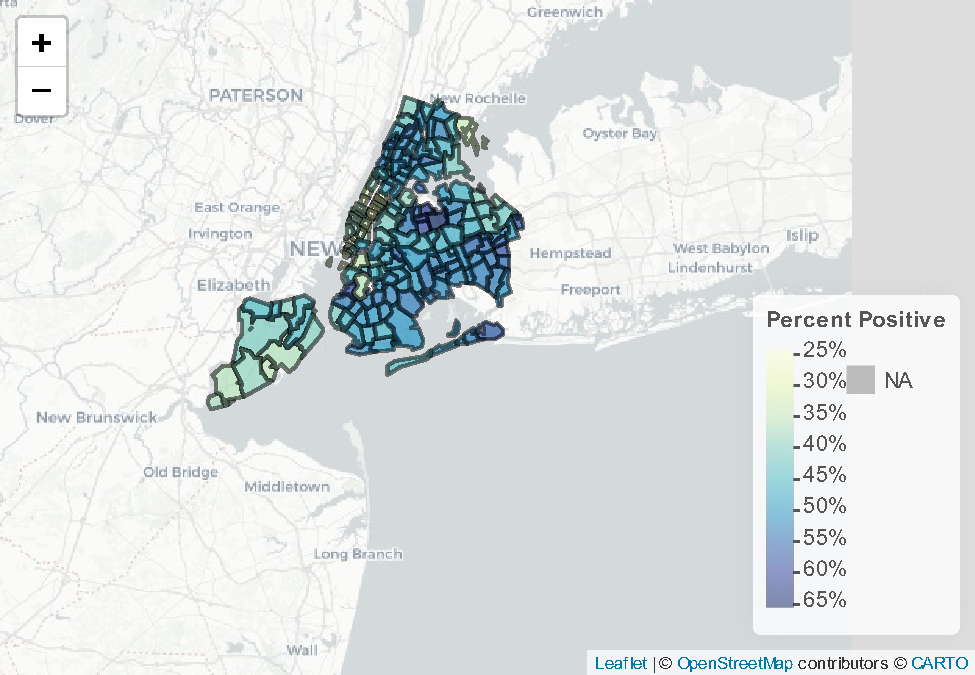
\includegraphics{leaflet_files/figure-latex/unnamed-chunk-12-1.pdf}
\#\#\#\# Leaflet\#4 - NYC CHILD OPP
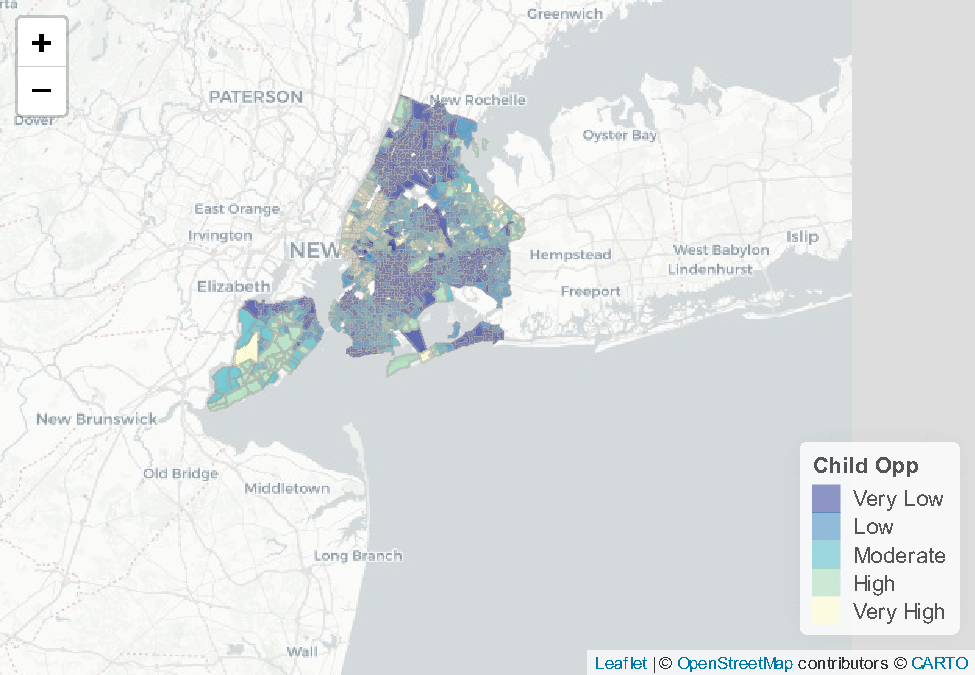
\includegraphics{leaflet_files/figure-latex/unnamed-chunk-13-1.pdf}
\#\#\#\# Leaflet\#5 - SVI by Census Tract + ZCTAS (ZIP) Overlay
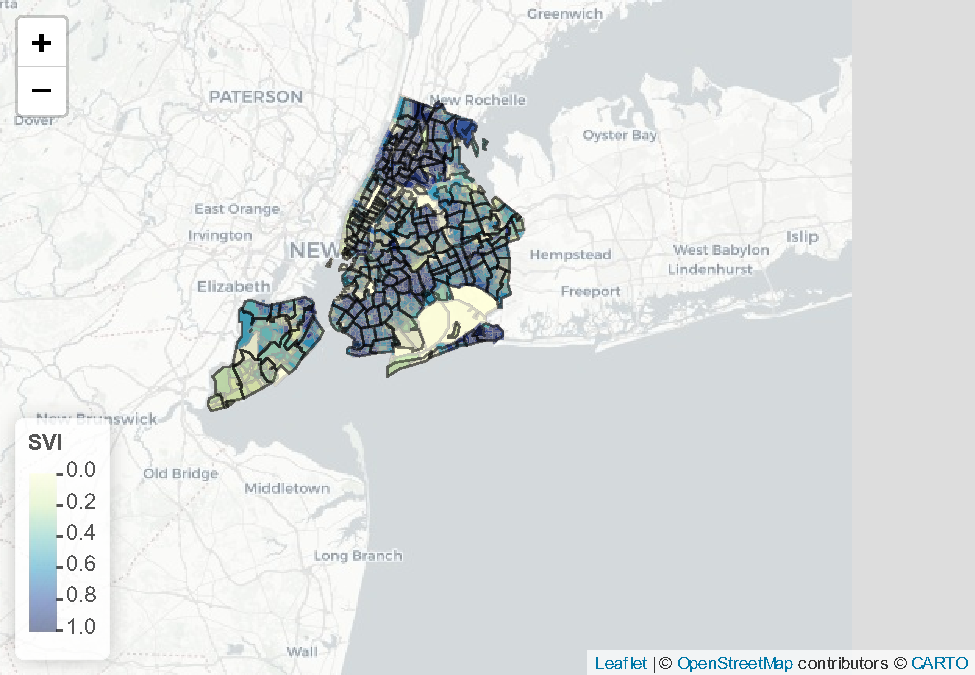
\includegraphics{leaflet_files/figure-latex/unnamed-chunk-14-1.pdf}

\end{document}
